\documentclass[12pt]{article}
 \usepackage[margin=1in]{geometry} 
\usepackage{amsmath,amsthm,amssymb,amsfonts,graphicx}
 
\newcommand{\N}{\mathbb{N}}
\newcommand{\Z}{\mathbb{Z}}
 
\newenvironment{problem}[2][Problem]{\begin{trivlist}
\item[\hskip \labelsep {\bfseries #1}\hskip \labelsep {\bfseries #2.}]}{\end{trivlist}}
%If you want to title your bold things something different just make another thing exactly like this but replace "problem" with the name of the thing you want, like theorem or lemma or whatever
 
\begin{document}
 
%\renewcommand{\qedsymbol}{\filledbox}
%Good resources for looking up how to do stuff:
%Binary operators: http://www.access2science.com/latex/Binary.html
%General help: http://en.wikibooks.org/wiki/LaTeX/Mathematics
%Or just google stuff
 
\title{CS189: Machine Learning\\
\large Homework 6: Neural Nets}
\author{Cameron Abrams}
\maketitle
 
\begin{problem}{1: Derivations}
For stochastic gradient descent we need to compute $\nabla_{W}L$ and $\nabla_{V}L$ where $L= -\sum_{j=1}^{K}y_{i}ln(z_{i}) +(1-y_{i})ln(1-z_{i})$ where $K$ is the number of classes. We will derive the gradients by their rows first.
$$\nabla_{W_{j}}L = \frac{\partial L}{\partial z_{j}}\frac{\partial z_{j}}{\partial w_{j}}=\frac{\partial L}{\partial z_{j}}\frac{\partial}{\partial w_{j}}s(W_{j}\cdot h)$$
$$\nabla_{W_{j}}L= \frac{\partial L}{\partial z_{j}}s(W_{j}\cdot h)(1-s(W_{j}\cdot h)h=\frac{\partial L}{\partial z_{j}}z_{j}(1-z_{j})h;$$
So we still need $\frac{\partial L}{\partial z_{j}}$, we'll come back and plug that in later.
$$\nabla_{V_{J}}L = \frac{\partial L}{\partial h_{j}}\frac{\partial h_{j}}{\partial V_{j}}=\frac{\partial L}{\partial h_{j}}\frac{\partial}{\partial V_{j}}(tanh(V_{j}\cdot x))
=\frac{\partial L}{\partial h_{j}}(1 - tanh^{2}(V_{j}\cdot x))
=\frac{\partial L}{\partial h_{j}}(1 - h_{j}^{2})x;$$
So we still need $\frac{\partial L}{\partial h_{j}}$. Let's derive $\frac{\partial L}{\partial z_{j}}$ and come back to that.
$$\frac{\partial L}{\partial z_{j}} = \frac{1-y_{j}}{1-z_{j}} - \frac{y_{j}}{z_{j}}.$$
So$$\nabla_{W_{j}}L = (z_{j}-y_{j})h$$
and thus, 
$$\nabla_{W}L = (z-y)h^{T}.$$
Let's derive $\frac{\partial L}{\partial h_{j}}$ now:
$$\frac{\partial L}{\partial h_{j}}=\frac{\partial}{\partial h_{j}}(-\sum_{i=1}^{K}y_{i}ln(s(W_{i}\cdot h)) +(1-y_{i})ln(1-s(W_{i}\cdot h)))$$
$$\frac{\partial L}{\partial h_{j}}=-\Big[\sum_{i=1}^{K}\Big(\frac{1-y_{j}}{1-z_{i}} - \frac{y_{i}}{z_{i}}\Big)z_{i}(1-z_{i})\Big]\frac{\partial}{\partial h_{j}}(W_i\cdot h)$$
$$\frac{\partial L}{\partial h_{j}}=-\sum_{i=1}^{K}(y_{i} - z_{i})\frac{\partial}{\partial h_{j}}(W_{i,1}h_1 + W_{i,2}h_2 \dots W_{i,m}h_{m})$$

$$\frac{\partial L}{\partial h_{j}}=-\sum_{i=1}^{K}(y_{i}-z_{i})W_{i,j}$$
$$\frac{\partial L}{\partial h_{j}}=\sum_{i=1}^{K}(z_{i}-y_{i})W_{i,j}.$$
Plugging into the equation above, we have:
$$\nabla_{V_{j}}L = \Big(\sum_{i=1}^{K}(z_{i}-y_{i})W_{i,j}\Big)(1-h_{j}^{2})x.$$
For $\nabla_{V_{j}}L$, this says the $j^{th}$ row of $\nabla_{V}L$ is the dot product of $z-y$ and $W_{j}$ multiplied by $1-h_{j}^{2}$ all scalar multiplied into the vector $x$. In matrix vector form, that is $$\nabla_{V}L = [W^{T}(z-y)\odot(1-h^{2})]x^{T}$$ where $\odot$ represents component-wise scalar multiplication.
\end{problem}

\newpage

\begin{problem}{2: Implementation}
I tuned the target values, the learning rates for $V$ and $W$, the decay rates for $V$ and $W$, and the batch size for mini-batch gradient descent. For my kaggle submission I settled on a batch size of $25$ samples, target values $0.1$ and $0.9$, learning rates $0.1$ and $0.01$, and decay rates $0.9$ and $0.6$ for $V$ and $W$ respectively which decayed every 4 epochs.\\
After 8 epochs I was able to achieve a training accuracy of $91\%$ and a validation accuracy of $86\%$.\\\\
This is a graph representing the value of the cost function of the predicted values at the $i^{th}$ iteration using stochastic gradient descent.
\begin{figure}[h]
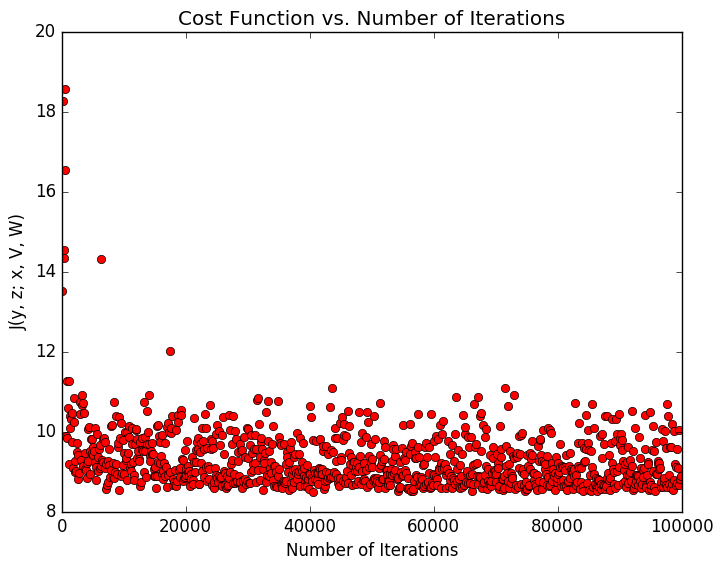
\includegraphics[totalheight=8cm]{Cost_Function.png}
\end{figure}
\begin{verbatim}
Kaggle Display Name: scoobyd
Kaggle Score: 0.86154
\end{verbatim}
\end{problem}

\newpage

\begin{problem}{3: Visualization}
Using a Neural Net that classified 88\% of the traning set images correctly and 86\% of the validation set images correctly here are 2 sets of 5 validation images that were classified.\\\\\\
5 images classified correctly:
\begin{figure}[h]

\includegraphics[totalheight=2cm]{images/correct0.png}

\includegraphics[totalheight=2cm]{images/correct1.png}

\includegraphics[totalheight=2cm]{images/correct2.png}

\includegraphics[totalheight=2cm]{images/correct3.png}

\includegraphics[totalheight=2cm]{images/correct4.png}
\end{figure}
\\5 images classfied incorrectly.
\begin{figure}[h]
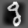
\includegraphics[totalheight=2cm]{images/incorrect0.png}
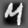
\includegraphics[totalheight=2cm]{images/incorrect1.png}

\includegraphics[totalheight=2cm]{images/incorrect2.png}

\includegraphics[totalheight=2cm]{images/incorrect3.png}

\includegraphics[totalheight=2cm]{images/incorrect4.png}
\end{figure}
\end{problem}

\newpage
\begin{problem}{4: Bells and Whistles}
\end{problem}
\newpage
\appendix
\section{\\NeuralNetwork.py}
\begin{verbatim}
import numpy as np
import scipy as sci

'''
Written by Cameron W.J. Abrams 4/13/2017
'''

# A Neural Network class that holds a trained Neural Network.
class NeuralNet:

	# IMAGES is a matrix of n samples points with 784 features, LABELS
	# is an array of n labels for each sample point and WEIGHT_DECAY
	# is an optional paramter used for regularization. 
	def __init__(self, images, labels, weight_decay=None):
		self.images = np.concatenate((images, np.ones((len(images[:,0]), 1))), axis=1)
		self.labels = labels
		self.weight_decay = weight_decay
		self.input_layer_size = 784
		self.hidden_layer_size = 200
		self.output_layer_size = 26
		mu = 0.0
		sigma_v = np.sqrt(1/self.input_layer_size)
		sigma_w = np.sqrt(1/self.hidden_layer_size)
		self.V = np.random.normal(mu, sigma_v, (self.hidden_layer_size, self.input_layer_size + 1))
		self.W = np.random.normal(mu, sigma_w, (self.output_layer_size, self.hidden_layer_size + 1))

	# The log loss function. Z,Y are predicted lables and lables respectively.
	def costFunction(self, z, y):
		for i in range(len(z)):
			if (z[i] == 0):
				z[i] == 10**-12
			elif (z[i] == 1):
				z[i] = 1 - 10**-12
		return -1*(np.dot(y.T, np.log(z)).ravel() + np.dot((1-y).T, np.log(1-z)).ravel())

	# The forward step of the Neural Network. Takes in a sample point, or batch of
	# sample points X and return a hidden layer H and predicted values Z.
	def forward(self, X):
		h = np.tanh(np.dot(self.V, X))
		h = np.insert(h, len(h), values=1, axis=0)
		z = sci.special.expit((np.dot(self.W, h)))
		return h, z

	# The backwards step of the Neural Network, takes in sample point, or batch
	# of sample points X, labels Y, hidden units H, and predicted values Z and
	# returns dJ/DV and dJdW (the gradients of the cost function w.r.t our weights.
	def backward(self, X, y, h, z):
		dJdV = np.dot(np.delete((np.dot(self.W.T, (z-y)) * (1 - h**2)), 200, axis=0), X.T)
		dJdW = np.dot((z-y), h.T)
		return dJdV, dJdW

	# The learn method is the gradient descent step. Takes in DJDV, DJDW,
	# the gradients of the the loss function w.r.t V and W. V_LEARNING_RATE
	#  and W_LEARNING_RATE are the learning rates for V and W respectively. 
	def learn(self, dJdV, dJdW, v_learning_rate, w_learning_rate):
		self.V = self.V - (v_learning_rate*dJdV)
		self.W = self.W - (w_learning_rate*dJdW)

	# Train method. Takes in V_LEARNING_RATE, W_LEARNING_RATE and trains
	# the data using those learning rates performing one full epoch through
	# the data.
	def train(self, v_learning_rate, w_learning_rate, randomized=False):
		for i in range(len(self.images)):
			if (randomized==True):
				j = np.random.randint(len(self.images))
			else:
				j = i
			x = (self.images[j, :]).reshape((len(self.images[0]), 1))
			y = self.labels[j,:].T.reshape(len(self.labels[0]), 1)
			h, z = self.forward(x)
			dJdV, dJdW = self.backward(x, y, h, z)
			self.learn(dJdV, dJdW, v_learning_rate=v_learning_rate, w_learning_rate=w_learning_rate)

	# TrainMini method. Takes in BATCH_SIZE, V_LEARNING_RATE, and W_LEARNING_RATE 
	# training the data using those learning rates performing one full epoch
	# through the data.
	def trainMini(self, batch_size, v_learning_rate, w_learning_rate):
		splits = len(self.images)//batch_size
		X = (self.images[:batch_size,:]).T
		Y = (self.labels[:batch_size,:]).T
		h,z = self.forward(X)
		dJdV, dJdW = self.backward(X, Y, h, z)
		self.learn((1/batch_size)*dJdV, (1/batch_size)*dJdW, v_learning_rate=v_learning_rate,
			w_learning_rate=w_learning_rate)
		for i in range(2,splits):
			X = (self.images[batch_size*(i-1):batch_size*i,:]).T
			Y = (self.labels[batch_size*(i-1):batch_size*i,:]).T
			h,z = self.forward(X)
			dJdV, dJdW = self.backward(X, Y, h, z)
			self.learn((1/batch_size)*dJdV, (1/batch_size)*dJdW, v_learning_rate=v_learning_rate,
				w_learning_rate=w_learning_rate)			
		X = (self.images[batch_size*splits:,:]).T
		Y = (self.labels[batch_size*splits:,:]).T
		h,z = self.forward(X)
		dJdV, dJdW = self.backward(X, Y, h, z)
		self.learn(dJdV*(1/batch_size), dJdW*(1/batch_size), v_learning_rate=v_learning_rate,
			w_learning_rate=w_learning_rate)

	# Same as the train method but returns two arrays, x_plot and y_plot where
	# the x_plot is the number of iterations and y_plot are the values of the
	# cost function at those iterations using the labels obtained by the Neural
	# Network at those points.
	def trainPlot(self, v_learning_rate, w_learning_rate, randomized=False):
		x_plot = list()
		y_plot = list()
		for i in range(len(self.images)):
			if (randomized==True):
				j = np.random.randint(len(self.images))
			else:
				j = i
			x = (self.images[j, :]).reshape((len(self.images[0]), 1))
			y = self.labels[j,:].T.reshape(len(self.labels[0]), 1)
			h, z = self.forward(x)
			dJdV, dJdW = self.backward(x, y, h, z)
			if (i % 100 == 0 and i != 0):
				x_plot.append(i)
				y_plot.append(self.costFunction(z, y))
			self.learn(dJdV, dJdW, v_learning_rate=v_learning_rate, w_learning_rate=w_learning_rate)
		return x_plot, y_plot

	# The classify method takes in a sample point X and returns a class 1-26.
	def classify(self, x):
		if (len(x) != len(self.V[0,:])):
			x = np.insert(x, len(x), values=1, axis=0)
		h = np.append(np.tanh(np.dot(self.V, x.T)), 1)
		z = sci.special.expit(np.dot(self.W, h))
		return np.argmax(z) + 1

	# The classifyAll method takes a matrix of images _IMAGES and returns
	# an list of classes 1-26 for each images.
	def classifyAll(self, _images):
		ret_arr = list()
		for i in range(len(_images)):
			ret_arr.append(self.classify(_images[i]))
		return ret_arr

	# Updates the Neural Networks images and labels. Used during training to
	# so that the training data can be reshuffled randomly and be fed back
	# to the Neural Network.
	def updateData(self, images, labels):
		self.images = np.concatenate((images, np.ones((len(images[:,0]), 1))), axis=1)
		self.labels = labels
\end{verbatim}
\newpage
\section{\\trainer.py}
\begin{verbatim}
from NeuralNetwork import NeuralNet
import numpy as np
import sklearn.preprocessing as skp
import matplotlib.pyplot as plt

'''
Written by Cameron W.J. Abrams 4/13/2017
'''

def main(target_values=None, epochs=8, v_learning_rate=0.1,
	w_learning_rate=0.01, v_decay_rate=1, w_decay_rate=1, randomized=False):

	_v_learning_rate = v_learning_rate
	_w_learning_rate = w_learning_rate
	images = np.load('data/images.npy')
	labels = np.load('data/vec_labels.npy')
	data = np.concatenate((images, labels), axis=1)
	np.random.shuffle(data)
	

	train_images = data[:round(.8*len(data)), :len(images[0])]
	train_labels = data[:round(.8*len(data)), len(images[0]):]
	validation_images = data[round(.8*len(data)):, :len(images[0])]
	validation_labels = data[round(.8*len(data)):, len(images[0]):]

	scaler = skp.StandardScaler()
	train_images = scaler.fit_transform(train_images)
	validation_images = scaler.transform(validation_images)

	# Set target values in our labels matrix(e.g. to 0.15 and 0.85).
	if target_values is not None:
		for i in range(len(train_labels[:,0])):
			for j in range(len(train_labels[0,:])):
				if train_labels[i,j] < 0.5:
					train_labels[i,j] = target_values[0]
				else:
					train_labels[i,j] = target_values[1]

	print('\n============\n  SETTINGS\n============')
	print('Target Values: ', target_values)
	print('Number of Epochs: ', epochs)
	print('V Learning Rate: ', v_learning_rate)
	print('W Learning Rate: ', w_learning_rate)
	print('V Decay Rate: ', v_decay_rate)
	print('W Decay Rate: ', w_decay_rate)
	print('Randomized: ', randomized)

	NN = NeuralNet(train_images, train_labels)

	for i in range(epochs):
		if (i > 0):
			data = np.concatenate((train_images, train_labels), axis=1)
			np.random.shuffle(data)
			train_images = data[:, :len(images[0])]
			train_labels = data[:, len(images[0]):]
			NN.updateData(train_images, train_labels)
			if ((i % 5) == 0):
				_v_learning_rate = v_decay_rate*v_learning_rate
				_w_learning_rate = w_decay_rate*w_learning_rate
		NN.train(v_learning_rate=_v_learning_rate, w_learning_rate=_w_learning_rate,
			randomized=randomized)

		print('\n============\n  EPOCH:', i, '\n============')

		# TRAINING ACCURACY
		y_hat = NN.classifyAll(train_images)
		test_correct = 0
		test_size = len(NN.images)
		for j in range(test_size):
			if (y_hat[j] == np.argmax(NN.labels[j]) + 1):
				test_correct += 1
			else:
				continue
		print('\nTest Classfication Complete:')
		print('Test Set Error: ', 1 - (test_correct / test_size))

		# VALIDATION ACCURACY
		total_correct = 0
		validation_size = len(validation_images)
		z = NN.classifyAll(validation_images)
		for j in range(len(z)):
			if (z[j] == np.argmax(validation_labels[j]) + 1):
				total_correct += 1
			else:
				continue
		print('\nValidation Classification Complete:')
		print('Validation Error Rate: ', 1 - (total_correct/validation_size), '\n')

if __name__ == '__main__':
	main(argv)
\end{verbatim}

\section{\\practice.py}
\begin{verbatim}
from trainer import main

'''
Written by Cameron W.J. Abrams 4/13/2017
'''

main(v_learning_rate=.1, w_learning_rate=.01, epochs=10)

\end{verbatim}

\newpage

\section{\\batch\_trainer.py}
\begin{verbatim}
from NeuralNetwork import NeuralNet
import numpy as np
import sklearn.preprocessing as skp

'''
Written by Cameron W.J. Abrams 4/13/2017
'''

def main(batch_size = 25, target_values=[0.1,0.9], epochs=7,
	v_learning_rate=0.1, w_learning_rate=0.01, v_decay_rate=1, w_decay_rate=1,
	decay_frequency=4):
	_v_learning_rate = v_learning_rate
	_w_learning_rate = w_learning_rate
	images = np.load('data/images.npy')
	labels = np.load('data/vec_labels.npy')
	data = np.concatenate((images, labels), axis=1)
	np.random.shuffle(data)
	
	train_images = data[:round(.8*len(data)), :len(images[0])]
	train_labels = data[:round(.8*len(data)), len(images[0]):]
	validation_images = data[round(.8*len(data)):, :len(images[0])]
	validation_labels = data[round(.8*len(data)):, len(images[0]):]

	scaler = skp.StandardScaler()
	train_images = scaler.fit_transform(train_images)
	validation_images = scaler.transform(validation_images)
	

	# Set target values in our labels matrix(e.g. to 0.15 and 0.85).
	if target_values is not None:
		for i in range(len(train_labels[:,0])):
			for j in range(len(train_labels[0,:])):
				if train_labels[i,j] < 0.5:
					train_labels[i,j] = target_values[0]
				else:
					train_labels[i,j] = target_values[1]

	print('\n============\n  SETTINGS\n============')
	print('Batch Size: ', batch_size)
	print('Target Values: ', target_values)
	print('Number of Epochs: ', epochs)
	print('V Learning Rate: ', v_learning_rate)
	print('W Learning Rate: ', w_learning_rate)
	print('V Decay Rate: ', v_decay_rate)
	print('W Decay Rate: ', w_decay_rate)
	print('Decay Frequency: ', decay_frequency)

	NN = NeuralNet(train_images, train_labels)

	for i in range(epochs):
		if (i > 0):
			data = np.concatenate((train_images, train_labels), axis=1)
			np.random.shuffle(data)
			train_images = data[:, :len(images[0])]
			train_labels = data[:, len(images[0]):]
			NN.updateData(train_images, train_labels)
			if ((i % decay_frequency) == 0):
				_v_learning_rate = v_decay_rate*_v_learning_rate
				_w_learning_rate = w_decay_rate*_w_learning_rate

		NN.trainMini(batch_size=batch_size,v_learning_rate=_v_learning_rate,
			w_learning_rate=_w_learning_rate)

		print('\n============\n  EPOCH:', i, '\n============')

		# TRAINING ACCURACY
		y_hat = NN.classifyAll(train_images)
		test_correct = 0
		test_size = len(NN.images)
		for j in range(test_size):
			if (y_hat[j] == np.argmax(NN.labels[j]) + 1):
				test_correct += 1
			else:
				continue
		print('\nTest Classfication Complete:')
		print('Test Set Error: ', 1 - (test_correct / test_size))

		# VALIDATION ACCURACY
		total_correct = 0
		validation_size = len(validation_images)
		z = NN.classifyAll(validation_images)
		for j in range(len(z)):
			if (z[j] == np.argmax(validation_labels[j]) + 1):
				total_correct += 1
			else:
				continue
		print('\nValidation Classification Complete:')
		print('Validation Error Rate: ', 1 - (total_correct/validation_size), '\n')

if __name__ == '__main__':
	main(argv)
\end{verbatim}
\section{\\practice.py}
\begin{verbatim}
from batch_trainer import main

'''
Written by Cameron W.J. Abrams 4/13/2017
'''

main(target_values=[0.05,0.95], epochs=48, v_decay_rate=0.9,
	w_decay_rate=0.6, decay_frequency=8)
\end{verbatim}

\newpage
\section{\\visualize.py}
\begin{verbatim}
from NeuralNetwork import NeuralNet
import numpy as np
import sklearn.preprocessing as skp
import matplotlib.pyplot as plt
import matplotlib.cm as cm

'''
Written by Cameron W.J. Abrams 4/13/2017
'''

images = np.load('data/images.npy')
labels = np.load('data/vec_labels.npy')
data = np.concatenate((images, labels), axis=1)
np.random.shuffle(data)

train_images = data[:round(.8*len(data)), :len(images[0])]
train_labels = data[:round(.8*len(data)), len(images[0]):]
validation_images = data[round(.8*len(data)):, :len(images[0])]
validation_labels = data[round(.8*len(data)):, len(images[0]):]

scaler = skp.StandardScaler()
train_images = scaler.fit_transform(train_images)
validation_images = scaler.transform(validation_images)

# Set target values in our labels matrix to 0.15 and 0.85
for i in range(len(train_labels[:,0])):
	for j in range(len(train_labels[0,:])):
		if train_labels[i,j] < 0.5:
			train_labels[i,j] = 0.1
		else:
			train_labels[i,j] = 0.9

# CREATE NeuralNet Object
NN = NeuralNet(train_images, train_labels)

# TRAIN NeuralNet Object
for i in range(5):
	if (i > 0):
		data = np.concatenate((train_images, train_labels), axis=1)
		np.random.shuffle(data)
		train_images = data[:, :len(images[0])]
		train_labels = data[:, len(images[0]):]
		NN.updateData(train_images, train_labels)
	NN.trainMini(batch_size=25, v_learning_rate=0.1, w_learning_rate=0.01)

correct_list = list()
incorrect_list = list()

# TRAINING ACCURACY
y_hat = NN.classifyAll(train_images)
test_correct = 0
test_size = len(NN.images)
for i in range(test_size):
	if (y_hat[i] == np.argmax(NN.labels[i]) + 1):
		test_correct += 1
	else:
		continue
print('\nTest Classfication Complete:')
print('Test Set Error: ', 1 - (test_correct / test_size))

# VALIDATION ACCURACY
total_correct = 0
validation_size = len(validation_images)
z = NN.classifyAll(validation_images)
for i in range(len(z)):
	if (z[i] == np.argmax(validation_labels[i]) + 1):
		total_correct += 1
		correct_list.append(validation_images[i])
	else:
		incorrect_list.append(validation_images[i])
		continue
print('\nValidation Classification Complete:')
print('Validation Error Rate: ', 1 - (total_correct/validation_size), '\n')

c_map = cm.get_cmap('Greys_r')

for i in range(5):
	plt.imsave('images/correct'+str(i), correct_list[i].reshape(28,28), cmap=c_map)
	plt.imsave('images/incorrect'+str(i), incorrect_list[i].reshape(28,28), cmap=c_map)
\end{verbatim}
\newpage
\section{\\cost\_plot.py}
\begin{verbatim}
from NeuralNetwork import NeuralNet
import scipy.io as sio
import numpy as np
import sklearn.preprocessing as skp
import matplotlib.pyplot as plt

'''
Written by Cameron W.J. Abrams 4/13/2017
'''

images = np.load('data/images.npy')
labels = np.load('data/vec_labels.npy')
data = np.concatenate((images, labels), axis=1)
np.random.shuffle(data)


train_images = data[:round(.8*len(data)), :len(images[0])]
train_labels = data[:round(.8*len(data)), len(images[0]):]
validation_images = data[round(.8*len(data)):, :len(images[0])]
validation_labels = data[round(.8*len(data)):, len(images[0]):]

scaler = skp.StandardScaler()
train_images = scaler.fit_transform(train_images)
validation_images = scaler.transform(validation_images)

# Set target values in our labels matrix to 0.15 and 0.85
for i in range(len(train_labels[:,0])):
	for j in range(len(train_labels[0,:])):
		if train_labels[i,j] < 0.5:
			train_labels[i,j] = 0.1
		else:
			train_labels[i,j] = 0.9

# CREATE NeuralNet Object
NN = NeuralNet(train_images, train_labels)

# TRAIN NeuralNet Object
for i in range(1):
	x_plot, y_plot = NN.trainPlot(v_learning_rate=0.01, w_learning_rate=0.001)
	# Plot of cost function vs number of iterations.
	plt.plot(x_plot, y_plot, 'ro')
	plt.xlabel('Number of Iterations')
	plt.ylabel('J(y, z; x, V, W)')
	plt.title('Cost Function vs. Number of Iterations')
	plt.savefig('Cost_Function.png', bbox_inches='tight')

# TRAINING ACCURACY
y_hat = NN.classifyAll(train_images)
test_correct = 0
test_size = len(NN.images)
for i in range(test_size):
	if (y_hat[i] == np.argmax(NN.labels[i]) + 1):
		test_correct += 1
	else:
		continue
print('\nTest Classfication Complete:')
print('Test Set Error: ', 1 - (test_correct / test_size))

# VALIDATION ACCURACY
total_correct = 0
validation_size = len(validation_images)
z = NN.classifyAll(validation_images)
for i in range(len(z)):
	if (z[i] == np.argmax(validation_labels[i]) + 1):
		total_correct += 1
	else:
		continue
print('\nValidation Classification Complete:')
print('Validation Error Rate: ', 1 - (total_correct/validation_size), '\n')
\end{verbatim}
\newpage
\section{\\kaggle\_submission.py}
\begin{verbatim}
from NeuralNetwork import NeuralNet
import scipy.io as sio
import numpy as np
import sklearn.preprocessing as skp

'''
Written by Cameron W.J. Abrams 4/13/2017
'''

images = np.load('data/images.npy')
labels = np.load('data/vec_labels.npy')
data = np.concatenate((images, labels), axis=1)
np.random.shuffle(data)

train_images = data[:, :len(images[0])]
train_labels = data[:, len(images[0]):]

scaler = skp.StandardScaler()
train_images = scaler.fit_transform(train_images)
test_data = np.load('data/test_data.npy')
test_data = scaler.transform(test_data)

# Set target values in our labels matrix(e.g. to 0.15 and 0.85).
for i in range(len(train_labels[:,0])):
	for j in range(len(train_labels[0,:])):
		if train_labels[i,j] < 0.5:
			train_labels[i,j] = .05
		else:
			train_labels[i,j] = .95

NN = NeuralNet(train_images, train_labels)

for i in range(8):
	if (i > 0):
		data = np.concatenate((train_images, train_labels), axis=1)
		train_images = data[:, :len(images[0])]
		train_labels = data[:, len(images[0]):]
		NN.updateData(train_images, train_labels)
	NN.trainMini(batch_size=50,v_learning_rate=0.1, w_learning_rate=0.01,
		v_decay_rate=1, w_decay_rate=1)

f = open('kaggle_submission.csv', 'w')
header = 'Id,Category\n'
f.write(header)

predictions = NN.classifyAll(test_data)
for i in range(len(test_data)):
	predicted_class = predictions[i]
	S = str(i + 1) + ',' + str(predicted_class) + '\n'
	f.write(S)
f.close()
\end{verbatim}
\end{document}